%!TEX root = tcc_proposta.tex
%----------------------------------------------------------------------------------
% Exemplo do uso da classe tcc.cls. Veja o arquivo .cls
% para mais detalhes e instruções.
%----------------------------------------------------------------------------------

%[ ] Literature Review: the literature review is meant to convey your knowledge of the subject matter of the proposal, so check for
    %[ ] Does it provide basic definitions of the area?
    %[ ] Terminology dropping from the sky: new technical terms must be explained before they are used, avoid talk about a deteronic frombotzer if you have not said what this is
    %[ ] Consistency of terminology: do not use different terms to refer to the same technical entity, once you define something as X always refer to it as X
    %[ ] Are the references up to date: i.e. do you cite work that was published in the last 5-10 years


\chapter{Fundamentação Teórica}\label{chap2:fund_teo}
    Antes de entender o trabalho desenvolvido, é importante que se explique os principais conceitos técnicos que servem de base para o desenvolvimento deste trabalho. Para tanto, descrevemos a metodologia utilizada para guiar nossa pesquisa, o que é um veículo de superfície não tripulado, as regulamentações de prevenção de colisões no mar, como realizar a evasão de colisão, e como se determina a identificação do ponto de maior aproximação.
    
    
    \section{Metodologia}
       Este trabalho foi realizado seguindo a seguinte metodologia: 
        
        \begin{enumerate}[label=\alph*)]
            \item \textbf{Identificação de um Problema de Pesquisa}: a partir da análise do trabalho de Jurak~\cite{Jurak2020COLREGS} foi possível observar que evasão de colisão aplicado a USV é uma demanda atual, e que determinar se um encontro entre duas embarcações resultará em colisão é uma necessidade em sistemas para USV. Com isso, originou-se a seguinte pergunta de pesquisa:
            
            \vspace{3mm}
            
            \centerline{\textit{"Como identificar situações de colisões no âmbito de USVs?"}}
            
            \item \textbf{Definição da Sentença de Busca}: a partir da pergunta formulada na etapa anterior, obteve-se o entendimento de quais áreas seriam permeadas para respondê-la. Com esse entendimento, extraiu-se as palavras chaves formulando a seguinte sentença de busca:
            
            \vspace{3mm}
            
            \centerline{\textit{"USV" AND "COLREGS" AND "collision avoidance"}}
            
            \item \textbf{Seleção de Trabalhos Relacionados}: aplicando a sentença de busca definida em bases de busca como IEEE Explorer\footnote{https://ieeexplore.ieee.org/Xplore/home.jsp}, Scopus\footnote{https://www.scopus.com/search/form.uri?display=basic} e Science Direct\footnote{https://www.sciencedirect.com/}, foi realizada uma pré-seleção de trabalhos que poderiam embasar o trabalho a ser realizado. A pré-seleção foi feita com base na leitura do resumo (\textit{"abstract"}) do trabalho e da dissertação acerca de evasão de colisão e CPA, resultando em 28 trabalhos pré-selecionados. Posteriormente, através de uma análise mais detalhada dos trabalhos, para identificar as técnicas utilizadas, e considerando seus respectivos Índice H, foram selecionados os 5 trabalhos mais relevantes que foram utilizados como referência neste trabalho.
            
            \item \textbf{Leitura dos Trabalhos Selecionados e Extração de Conhecimentos Relevantes}: para obter um conhecimento mais aprofundado a respeito da área, do problema e das técnicas utilizadas pelos autores atualmente, foi realizada a leitura completa dos trabalhos atentando para a fundamentação teórica e analisando brevemente seus resultados. Com isso foi possível compreender como implementar CPA e quais resultados esperar da implementação.
            
            \item \textbf{Estruturação da Proposta de Trabalho}: com o conhecimento obtido da etapa anterior foi possível estruturar uma proposta de trabalho contendo uma contextualização, embasamento teórico, objetivos e os meios que serão utilizados para atingi-los.
            
            \item \textbf{Implementação da Proposta Aceita}: com a proposta analisada e aprovada pelos avaliadores, realizou-se a implementação do CPA e a integração com o sistema desenvolvido por Jurak~\cite{Jurak2020COLREGS}.
            
            \item \textbf{Execução Casos de Testes}: realizamos a validação da nossa implementação através de simulação, onde realizamos os mesmos casos de testes executados por Jurak~\cite{Jurak2020COLREGS} com a finalidade de verificar o impacto de nossa implementação no sistema base. Além disso, realizamos casos de testes específicos onde buscamos evidenciar nossa contribuição.
            
            \item \textbf{Análise dos Resultados}: analisamos o comportamento obtido na fase de testes e comparamos com o comportamento anterior à implementação deste trabalho.
        \end{enumerate}
    
    \section{Veículo de Superfície Não Tripulado}\label{subchap2:USV}
        Um veículo de superfície não tripulado (do inglês \textit{"Unmanned Surface Vehicle"} - USV) é caracterizado por realizar atividades navais de forma autônoma, ou controlado remotamente, sem a presença de tripulação~\cite{Liu2016Unmanned}. Tais características também enquadram um USV na categoria de um robô~\cite{Jurak2020COLREGS}.
        De acordo com Liu \etal~\cite{Liu2016Unmanned}, um USV pode ter as mais variadas aparências e funcionalidades, porém os seguintes componentes básicos devem compor um USV: 
        \begin{enumerate*}[label=\alph*)]
            \item casco e estruturas mecânicas auxiliares;
            \item sistema de propulsão;
            \item sistema de orientação, navegação e controle (do inglês \textit{"Guidance Navigation and Control"} - GNC);
            \item sistema de comunicação;
            \item equipamento de coleta de dados;
            \item estação de solo.
        \end{enumerate*}
        
        Dentre os elementos listados o sistema GNC é fundamental para automatizar uma embarcação, pois ele controlará a embarcação como um todo. Segundo Fossen~\cite{Fossen2011Handbook}, um sistema GNC consiste em controlar automaticamente ou remotamente dispositivos ou veículos. Sua função consiste em coletar informações a respeito da embarcação e seu entorno (\textit{Navigation}), gerenciar dados de missão encontrando o caminho necessário para completá-la (\textit{Guidance}) e executar as ações necessárias para atingir o objetivo desejado (\textit{Control})~\cite{Liu2016Unmanned}. A Figura ~\ref{fig:Liu2016_gncSystem}, criada com base em Liu \etal~\cite{Liu2016Unmanned}, mostra o sistema GNC de forma simplificada, apontando algumas de suas funcionalidades. Tais funções serão brevemente explicadas a seguir.
        
        \begin{figure}
            \centering
            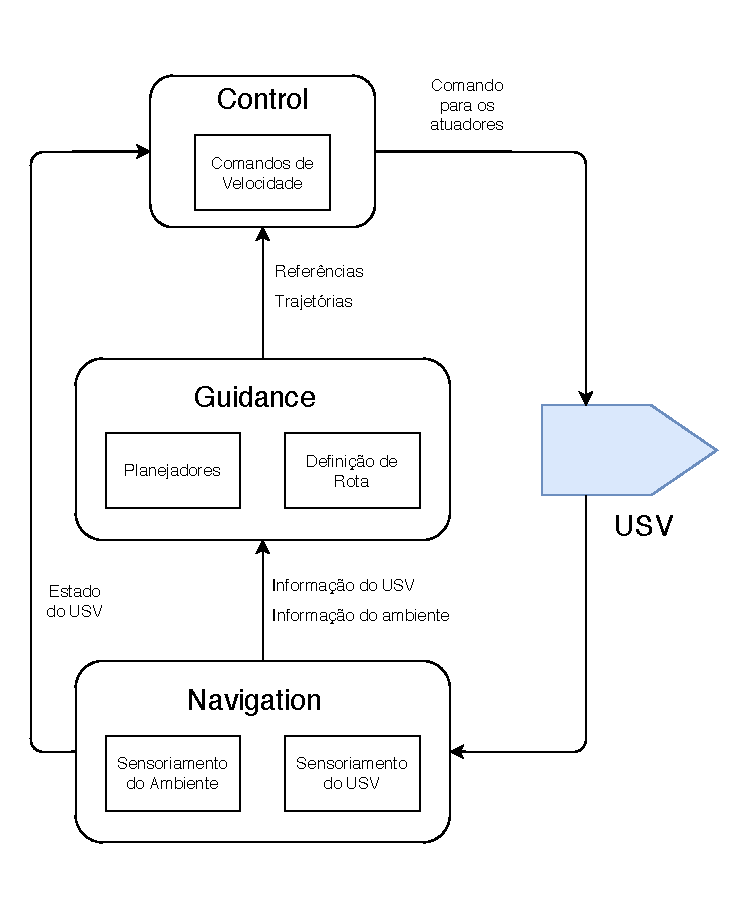
\includegraphics[width=0.8\textwidth]{fig/chap2/sistema_gnc_liu.pdf}
            \caption{Detalhamento do sistema GNC com suas respectivas funções (Imagem baseada em Liu~\etal~\cite{Liu2016Unmanned}).}
            \label{fig:Liu2016_gncSystem}
        \end{figure}
        
        \begin{enumerate}
            \item \textit{"Navigation":} subsistema responsável pela coleta de informações a respeito do barco (posição, velocidade, \etc) e seu entorno (obstáculos estáticos e obstáculos móveis). Essas informações são coletadas por meio de sensores, radares, câmeras, cartas náuticas e mapas. Os dados coletados são enviados para o subsistema \textit{"Guidance"} e \textit{"Control"}.
            
            \item \textit{"Guidance":} subsistema responsável por gerenciar os dados da missão atual a ser executada e definir os meios necessários para cumpri-la. Através dos dados obtidos do subsistema \textit{"Navigation"}, as ações necessárias para atingir o objetivo são definidas e enviadas para o subsistema \textit{"Control"}.
            
            \item \textit{"Control":} subsistema que, com base no estado atual da embarcação obtido pelo subsistema \textit{"Navigation"}, gera os comandos necessários para realizar as ações definidas pelo subsistema \textit{"Guidance"}. Além disso, também é sua responsabilidade executar os comandos gerados diretamente nos atuadores da embarcação.
        \end{enumerate}
        
        Visto que o escopo de desenvolvimento deste trabalho é em evasão de colisão, focaremos no subsistema responsável por tal função: o subsistema de \textit{"Guidance"}. Sua implementação consiste em, além do gerenciamento dos dados de missão, estabelecer qual a melhor rota para o USV percorrer~\cite{Jurak2020COLREGS}. A definição da rota geralmente ocorre em dois níveis: global e local. Ambos os níveis utilizam planejadores; o planejador global definirá a rota a ser corrida em um mapa de larga escala, chamada de rota global, considerando obstáculos estáticos conhecidos; já o planejador local atentará para o surgimento de obstáculos que não foram considerados na rota global e que precisarão ser desviados, desviando da rota global momentaneamente através de uma rota local específica para a atual situação~\cite{Liu2016Unmanned}.
    
    \section{Regulamentações de Prevenção de Colisões no Mar}\label{subchap2:colregs}
        Buscando padronizar as ações tomadas para evitar colisões, a Organização Internacional da Marinha (IMO - do inglês \textit{"International Marine Organization"}) definiu as regulamentações de prevenção de colisões no mar (COLREGS - do inglês \textit{"COLlision REGulations at Sea"})~\cite{COLREGS}.
        Para que o uso de USV não apresente perigo para outras embarcações, sendo elas tripuladas ou não, é necessário que ele realize ações conhecidas e esperadas pela embarcação que se aproxima. Sendo assim, o USV deverá realizar suas ações de acordo com as COLREGS de forma que seja perceptível para a outra embarcação~\cite{Kuwata2014Safe}. Jurak~\cite{Jurak2020COLREGS} em seu sistema considerou os encontros \textit{"head-on"}, \textit{"crossing from left"}, \textit{"crossing from right"} e \textit{"overtake"}. As situações listadas são ilustradas na Figura~\ref{fig:Jurak2020COLREGS_colregsSituations} e explicadas a seguir. 
        
        \begin{figure}
            \centering
            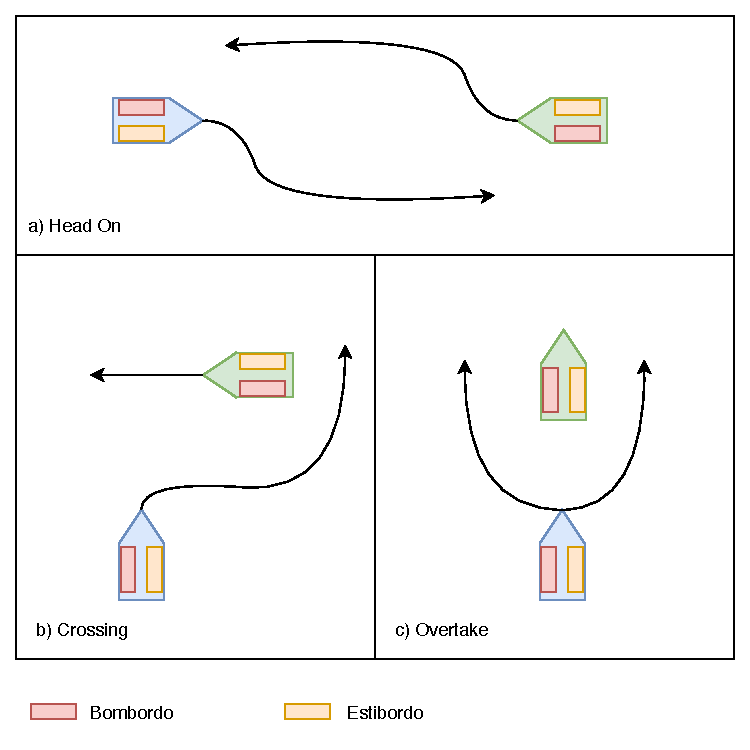
\includegraphics[width=\textwidth]{fig/chap2/encontros_colregs.pdf}
            \caption{Tipos de encontros entre embarcações previstos pelas COLREGS~\cite{Jurak2020COLREGS}.}
            \label{fig:Jurak2020COLREGS_colregsSituations}
        \end{figure}
        
        \begin{enumerate}[label=\alph*]
            \item \textit{"Head-on":} situação em que as embarcações se encontram frente a frente. Nesse caso, as COLREGS especificam que ambas as embarcações devem evitar a colisão virando à direita  (\textit{"starboard side"} - estibordo) e, por consequência, passando pelo lado esquerdo (\textit{"port side"} - bombordo) da outra embarcação.
            
            \item \textit{"Crossing from left/right":} situação em que uma embarcação cruzará o caminho da outra. Nesse caso, a embarcação que encontrar a outra no seu lado direito (\textit{"startboard side"} - estibordo) é responsável por evitar a colisão contornando a embarcação que se aproxima por trás, realizando uma conversão à direita (\textit{"startboard"} - estibordo). Já a embarcação que possuir a outra no seu lado esquerdo (\textit{"port side"} - bombordo), não deverá mudar seu curso.
            
            \item \textit{"Overtaking":} situação em que uma embarcação se encontra em uma velocidade maior do que a embarcação que se encontra à frente. Nesse caso a embarcação que se aproxima deve desviar pelo lado em que não causará uma nova situação de \textit{"overtaking"}.
        \end{enumerate}
    
    \section{Evasão de Colisão}\label{subchap2:prev_col}
        Uma tarefa primordial quando se trata de navegação é evitar que a embarcação colida com algum obstáculo e outras embarcações. Entretanto, prevenção de colisão consiste em um dos principais desafios ao desenvolver um USV~\cite{Jurak2020COLREGS}. Em um USV o sistema GNC é responsável por realizar todo o procedimento de prevenção de colisão, sendo o subsistema \textit{"Guidance"} o encarregado de detectar a colisão e encontrar uma solução para que ela não ocorra~\cite{Huang2020Ship}.
        Huang \etal~\cite[p.451]{Huang2020Ship} define prevenção de colisão como: \textit{"Prevenção de colisão é o processo em que uma embarcação desvia de sua trajetória planejada para evitar contato físico indesejado em um certo tempo futuro."} Com isso, Huang \etal~\cite{Huang2020Ship} separa o processo de prevenção de colisão nas seguintes etapas: 
        
        \begin{enumerate}
            \item \textbf{Previsão de Movimento}: que prevê estados futuros do USV e de todas as outras embarcações envolvidas no encontro;
            \item \textbf{Detecção de Conflito}: determina se o USV está em risco de colisão;
            \item \textbf{Resolução de Conflito}: encontrará o melhor caminho para evitar a colisão.
        \end{enumerate}
        
        A Figura~\ref{fig:Huang2020_collisionAvoidanceProcess}, feita com base em Huang \etal~\cite{Huang2020Ship}, mostra o fluxo de informação realizada em um sistema GNC no procedimento de prevenção de colisão. Na imagem, podemos considerar \textit{"Observer"} e \textit{"Actuator"} como módulos dos subsistemas de \textit{"Navigation"} e \textit{"Control"}, respectivamente. Os módulos envoltos pelo pontilhado vermelho correspondem às etapas listadas anteriormente e são de responsabilidade do subsistema \textit{"Guidance"}. As informações coletadas pelo \textit{"Observer"} são utilizadas pelo módulo \textit{"Motion Prediction"}, quando implementado, para realizar as previsões necessárias. O módulo \textit{"Conflict Detection"} utilizará as informações providas pelo \textit{"Motion Prediction"}, e/ou \textit{"Observer"}, a fim de identificar se há risco de colisão. Se não houver, as diretivas de caminho e velocidade são enviadas diretamente para o \textit{"Actuator"}. Caso haja risco de colisão, o módulo \textit{"Conflict Resolution"} será acionado para que encontre um caminho seguro para evitar a colisão, consequentemente, gerando diretivas de caminho e velocidade que levarão a um desvio momentâneo da rota global.
        
        \begin{figure}[H]
            \centering
            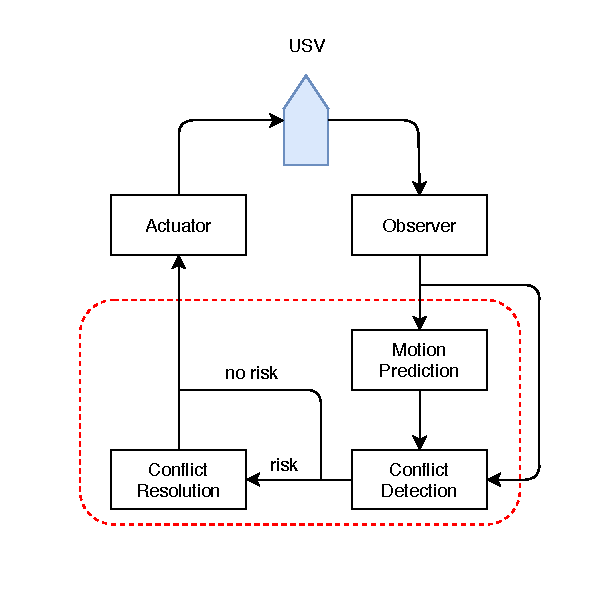
\includegraphics{fig/chap2/fluxo_de_informação.pdf}
            \caption{Fluxo de informação em um sistema GNC no procedimento de prevenção de colisão (Imagem baseada em Huang~\etal~\cite{Huang2020Ship}).}
            \label{fig:Huang2020_collisionAvoidanceProcess}
        \end{figure}
        
    \section{Ponto de Maior Aproximação}\label{subchap2:cpa}
        Um meio popular de se avaliar o Índice de Risco de Colisão (do inglês \textit{"Collision Risk Index"} - CRI) é através do método de Ponto de Maior Aproximação (do inglês \textit{"Closest Point of Approach"} -  CPA)~\cite{Huang2020Ship}. Nele, dois indicadores são considerados: Distância no ponto de maior aproximação (DCPA - do inglês \textit{"Distance to Closest Point of Approach"}), e Tempo para o Ponto de Maior Aproximação (TCPA - do inglês \textit{"Time to Closest Point of Approach"})~\cite{Huang2019Generalized}. Ambos indicadores são valores numéricos e contribuem para a detecção de uma situação de risco de colisão. Quando os valores resultantes atingirem um limiar (\textit{"threshold"}), é detectado um risco de colisão eminente e o procedimento para evitar o acidente é iniciado~\cite{Huang2020Ship}. 
        
        Segundo Kuwata~\etal~\cite{Kuwata2014Safe}, a partir da posição \pos e da velocidade \vel das embarcações é possível obter o \tcpa através da equação~\eqref{eq:tcpa}, e o \dcpa através da equação~\eqref{eq:dcpa}. Utilizaremos os indicadores \tcpa e \dcpa para identificar encontros em que a COLREGS deve ser aplicada. Se os valores obtidos satisfizerem a condição descrita na Desigualdade~\eqref{eq:cpaThreshold}, é preciso evadir da colisão de acordo com a COLREGS aplicável ao encontro~\cite{Kuwata2014Safe}. Para este trabalho consideramos $t_{max} = 20s$ e $d_{min} = 9m$.
        % Comentário para evitar novo parágrafo
        \begin{align}
            t_{\rm CPA} &=
            \begin{cases}
                0, & \text{if } \Vert\vec{v}_{A}-\vec{v}_{B}\Vert\leq\epsilon\\
                \displaystyle{{(\vec{p}_{A}-\vec{p}_{B})\cdot(\vec{v}_{A}-\vec{v}_{B})}\over{\Vert\vec{v}_{A}-\vec{v}_{B}\Vert^{2}}}
            \end{cases}\label{eq:tcpa}\\
            d_{\rm CPA} &=\bigl\Vert (\vec{p}_{A}+\vec{v}_{A}t_{\rm CPA})-(\vec{p}_{B}+\vec{v}_{B}t_{\rm CPA})\bigr\Vert\label{eq:dcpa}
        \end{align}
        
        \begin{equation}\label{eq:cpaThreshold}
            0\leq t_{\rm CPA}\leq t_{\max}\quad{\hbox {and}}\quad d_{\rm CPA}\leq d_{\min}
        \end{equation}
    
        Para obter um maior entendimento de como é possível analisar os estados futuros das embarcações para avaliar o risco de colisão a partir da Equação~\ref{eq:tcpa}, explicaremos visualmente. Consideremos um USV cuja posição é $\vec{p}_{A}(1,1)$ e uma outra embarcação $\mathcal{B}$ cuja posição é $\vec{p}_{B}(7,1)$. Consideremos também que a velocidade do USV é $\vec{v}_{A}(1,1)$ e que a velocidade da embarcação $\mathcal{B}$ é $\vec{v}_{B}(-1,1)$, como mostrado na Figura~\ref{fig:chap2_scenario}.
        Primeiramente verifiquemos se $\Vert\vec{v}_{A}-\vec{v}_{B}\Vert\leq\epsilon$ e, caso a verificação seja verdadeira, consideraremos $t_{CPA} = 0$. Isso é para evitar que o denominador da Equação~\ref{eq:tcpa} resulte em um número muito pequeno, fazendo com que o \tcpa resulte em um número muito grande, além de garantir que não haverá uma divisão por zero. Porém neste caso temos que $\Vert\vec{v}_{A}-\vec{v}_{B}\Vert = 4$, logo, podemos calcular o \tcpa de acordo com o segundo caso da Equação~\ref{eq:tcpa}. Calculando a posição e a velocidade relativa das embarcações temos que $\vec{p}_{A}-\vec{p}_{B} = (-6,0)$ e que $\vec{v}_{A}-\vec{v}_{B} = (2,0)$, respectivamente. Essas operações são ilustradas pela Figura~\ref{fig:chap2_pa_pb} e pela Figura~\ref{fig:chap2_va_vb}, respectivamente. Com os vetores resultantes podemos realizar o produto escalar $(-6,0)\cdot(2,0) = -12$, que aplicado na Equação~\ref{eq:tcpa} resulta em $t_{CPA} = -3$.
    
        \begin{figure}[H]
            \centering
            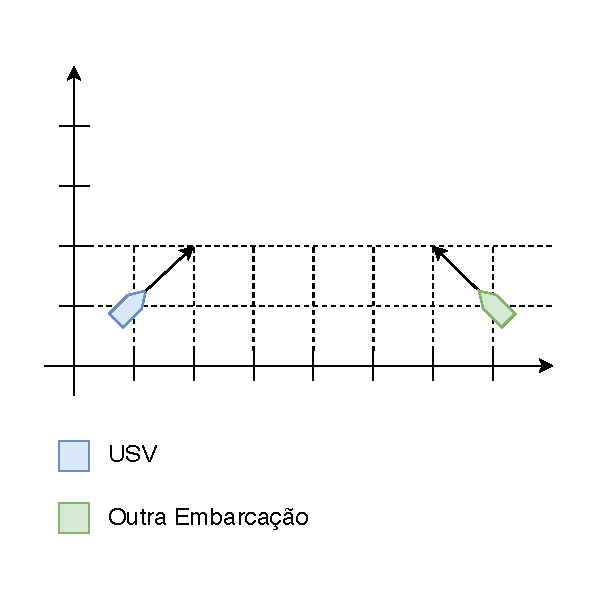
\includegraphics{fig/chap2/cpa_example_scenario.pdf}
            \caption{Cenário inicial do exemplo apresentado.}
            \label{fig:chap2_scenario}
        \end{figure}
        
        \begin{figure}
            \centering
            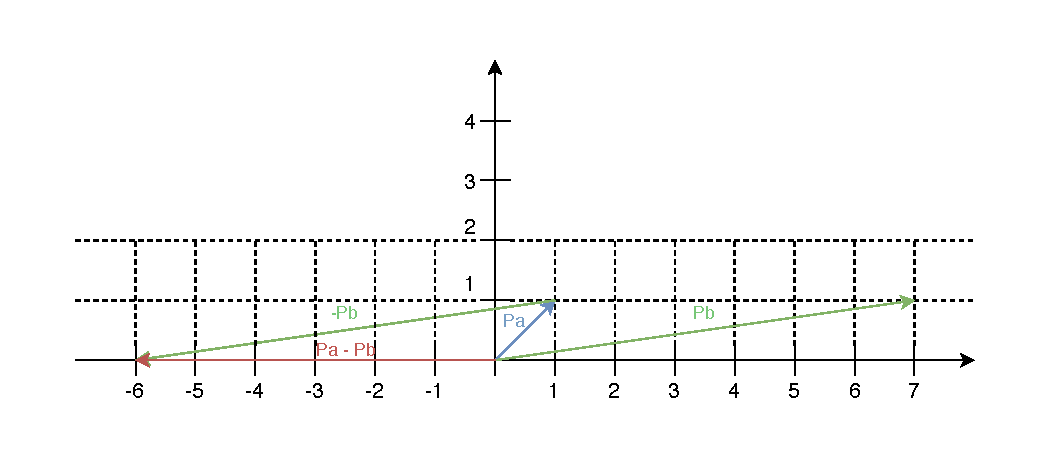
\includegraphics{fig/chap2/cpa_explanation_pa_pb.pdf}
            \caption{Operação vetorial $\vec{p}_{A}-\vec{p}_{B}$}
            \label{fig:chap2_pa_pb}
        \end{figure}
        
        \begin{figure}
            \centering
            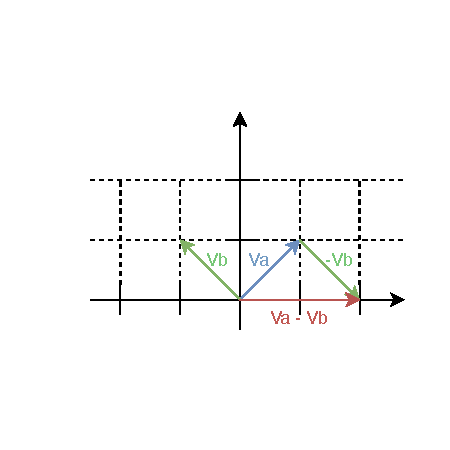
\includegraphics[scale=1.5]{fig/chap2/cpa_explanation_va_vb.pdf}
            \caption{Operação vetorial  $\vec{v}_{A}-\vec{v}_{B}$}
            \label{fig:chap2_va_vb}
        \end{figure}
        
        Com o \tcpa calculado, podemos obter o \dcpa. A Equação~\ref{eq:dcpa} coloca que os vetores velocidade das embarcações devem ser multiplicados pelo \tcpa encontrado. Apesar de Kuwata~\etal~\cite{Kuwata2014Safe} não indicar explicitamente o uso do valor absoluto do \tcpa encontrado, optamos por fazê-lo dado que se multiplicássemos as velocidades por um \tcpa negativo, estaríamos invertendo o sentido das velocidades, o que não é desejável, dado que o \tcpa é utilizado no cálculo do \dcpa para estender o vetor velocidade da embarcação, partindo da sua posição, até o ponto de maior proximidade. Posto isso, ao aplicarmos a Equação~\ref{eq:dcpa} para ambas as embarcações, temos os pontos em que cada uma delas estarão no momento em que estiverem mais próximas uma da outra, para que seja calculada a distância entre elas. 
      
        Para ilustrar o cálculo do \dcpa, daremos continuidade ao exemplo apresentado até então. Aplicando os vetores posição e os vetores velocidade das embarcações, já multiplicados pelo valor absoluto do \tcpa, na Equação~\ref{eq:dcpa} temos que $\Vert (1+3,1+3)-(7-3,1+3)\Vert = 0$. Essa é a distância entre as embarcações no ponto de maior proximidade, ou seja, certamente haverá colisão. Na Figura~\ref{fig:chap2_collision} apresentamos as embarcações em suas posições iniciais e estendemos o vetor velocidade \tcpa vezes, indicando onde cada embarcação estaria em cada instante de tempo. É possível observar que no terceiro instante de tempo as embarcações estariam ocupando a mesma posição, ou seja, a distância entre elas seria zero.
        
        \begin{figure}[H]
            \centering
            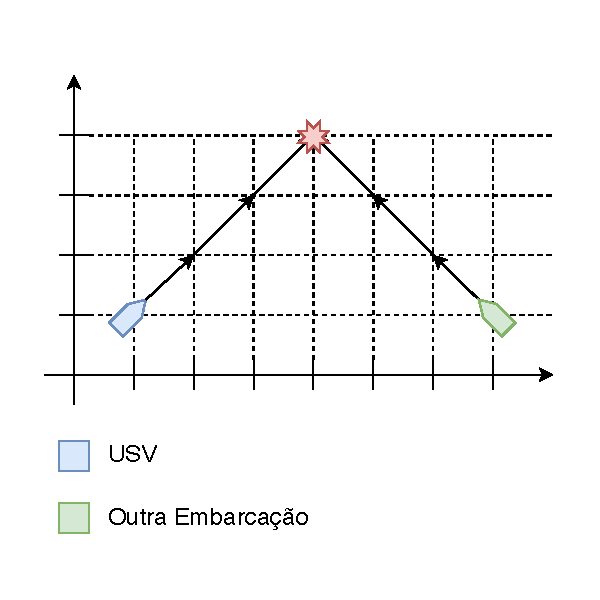
\includegraphics{fig/chap2/cpa_explanation_collision.pdf}
            \caption{Ilustração do CPA calculado - Exemplo 1}
            \label{fig:chap2_collision}
        \end{figure}
        
        Em um segundo exemplo, consideremos as mesmas condições iniciais do exemplo anterior alterando apenas a velocidade da outra embarcação para $\vec{v}_{B}(-0.5,-0.5)$. Nesse caso, realizando os mesmos cálculos, temos que $t_{CPA} = 3.6s$ e $d_{CPA} = 1.9m$. Isso significa que no ponto de maior proximidade a distância entre as embarcações será de 1.9m. A Figura~\ref{fig:chap2_almost_collision} apresenta informações 
        análogas à Figura~\ref{fig:chap2_collision}, com a única diferença sendo o ponto azul indicando a posição do USV no tempo t = \tcpa e o ponto verde indicando a posição da outra embarcação no tempo t = \tcpa. Com essas informações, é possível determinar se essa é uma 
        situação de risco ou não. Se for uma situação de risco é necessário evadir de acordo com as COLREGS, caso contrário a evasão não é necessária.
        
        \begin{figure}
            \centering
            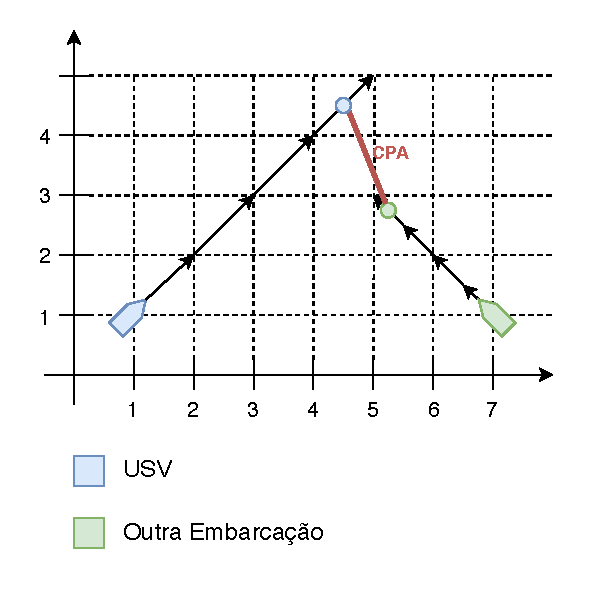
\includegraphics{fig/chap2/cpa_explanation_almost_collision.pdf}
            \caption{Ilustração do CPA calculado - Exemplo 2}
            \label{fig:chap2_almost_collision}
        \end{figure} 